% -*- coding: utf-8 -*-
%-------------------------designed by zcf--------------
\documentclass[UTF8,a4paper,10pt]{ctexart}
\usepackage[left=3.17cm, right=3.17cm, top=2.74cm, bottom=2.74cm]{geometry}
\usepackage{amsmath}
\usepackage{graphicx,subfig}
\usepackage{float}
\usepackage{subcaption} 
\usepackage{cite}
\usepackage{caption}
\usepackage{enumerate}
\usepackage{booktabs} % 表格
\usepackage{multirow}
\newcommand{\tabincell}[2]{
\begin{tabular}{@{}#1@{}}#2\end{tabular}
}  % 表格强制换行
%-------------------------字体设置--------------
\usepackage{ctex}
\setCJKmainfont[ItalicFont=Noto Sans CJK SC Bold, BoldFont=Noto Serif CJK SC Black]{Noto Serif CJK SC}
\newcommand{\yihao}{\fontsize{26pt}{36pt}\selectfont}           % 一号, 1.4 倍行距
\newcommand{\erhao}{\fontsize{22pt}{28pt}\selectfont}          % 二号, 1.25倍行距
\newcommand{\xiaoer}{\fontsize{18pt}{18pt}\selectfont}          % 小二, 单倍行距
\newcommand{\sanhao}{\fontsize{16pt}{24pt}\selectfont}  % 三号字
\newcommand{\xiaosan}{\fontsize{15pt}{22pt}\selectfont}        % 小三, 1.5倍行距
\newcommand{\sihao}{\fontsize{14pt}{21pt}\selectfont}            % 四号, 1.5 倍行距
\newcommand{\banxiaosi}{\fontsize{13pt}{19.5pt}\selectfont}    % 半小四, 1.5倍行距
\newcommand{\xiaosi}{\fontsize{12pt}{18pt}\selectfont}            % 小四, 1.5倍行距
\newcommand{\dawuhao}{\fontsize{11pt}{11pt}\selectfont}       % 大五号, 单倍行距
\newcommand{\wuhao}{\fontsize{10.5pt}{15.75pt}\selectfont}    % 五号, 单倍行距
%-------------------------章节名----------------
\usepackage{ctexcap} 
\CTEXsetup[name={,、},number={ \chinese{section}}]{section}
\CTEXsetup[name={(,)},number={\chinese{subsection}}]{subsection}
\CTEXsetup[name={,.},number={\arabic{subsubsection}}]{subsubsection}
%-------------------------页眉页脚--------------
\usepackage{fancyhdr}
\pagestyle{fancy}
\lhead{\kaishu \leftmark}
\rhead{\kaishu 实验报告}% 加粗\bfseries 
\lfoot{}
\cfoot{\thepage}
\rfoot{}
\renewcommand{\headrulewidth}{0.1pt}  
\renewcommand{\footrulewidth}{0pt}% 去掉横线
\newcommand{\HRule}{\rule{\linewidth}{0.5mm}}% 标题横线
\newcommand{\HRulegrossa}{\rule{\linewidth}{1.2mm}}
%-----------------------伪代码------------------
\usepackage{algorithm}  
\usepackage{algorithmicx}  
\usepackage{algpseudocode}  
\floatname{algorithm}{Algorithm}  
\renewcommand{\algorithmicrequire}{\textbf{Input:}}  
\renewcommand{\algorithmicensure}{\textbf{Output:}} 
\usepackage{lipsum}  
\makeatletter
\newenvironment{breakablealgorithm}
  {% 
\begin{breakablealgorithm}
  \begin{center}
     \refstepcounter{algorithm}% New algorithm
     \hrule height.8pt depth0pt \kern2pt% \@fs@pre for \@fs@ruled
     \renewcommand{\caption}[2][\relax]{% Make a new \caption
      {\raggedright\textbf{\ALG@name~\thealgorithm} ##2\par}%
      \ifx\relax##1\relax % #1 is \relax
         \addcontentsline{loa}{algorithm}{\protect\numberline{\thealgorithm}##2}%
      \else % #1 is not \relax
         \addcontentsline{loa}{algorithm}{\protect\numberline{\thealgorithm}##1}%
      \fi
      \kern2pt\hrule\kern2pt
     }
  }{% \end{breakablealgorithm}
     \kern2pt\hrule\relax% \@fs@post for \@fs@ruled
  \end{center}
  }
\makeatother
%------------------------代码-------------------
\usepackage{xcolor} 
\usepackage{listings} 
\lstset{ 
breaklines,% 自动换行
basicstyle=\small,
escapeinside=``,
keywordstyle=\color{ blue!70} \bfseries,
commentstyle=\color{red!50!green!50!blue!50},% 
stringstyle=\ttfamily,% 
extendedchars=false,% 
linewidth=\textwidth,% 
numbers=left,% 
numberstyle=\tiny \color{blue!50},% 
frame=trbl% 
rulesepcolor= \color{ red!20!green!20!blue!20} 
}
%------------超链接----------
\usepackage[colorlinks,linkcolor=black,anchorcolor=blue]{hyperref}
%------------------------TODO-------------------
\usepackage{enumitem,amssymb}
\newlist{todolist}{itemize}{2}
\setlist[todolist]{label=$\square$}
\usepackage{pifont}
\newcommand{\cmark}{\ding{51}}%
\newcommand{\xmark}{\ding{55}}%
\newcommand{\done}{\rlap{$\square$}{\raisebox{2pt}{\large\hspace{1pt}\cmark}}\hspace{-2.5pt}}
\newcommand{\wontfix}{\rlap{$\square$}{\large\hspace{1pt}\xmark}}
%------------------------水印-------------------
\usepackage{tikz}
\usepackage{xcolor}
\usepackage{eso-pic}

\newcommand{\watermark}[3]{\AddToShipoutPictureBG{
\parbox[b][\paperheight]{\paperwidth}{
\vfill%
\centering%
\tikz[remember picture, overlay]%
  \node [rotate = #1, scale = #2] at (current page.center)%
    {\textcolor{gray!80!cyan!30!magenta!30}{#3}};
\vfill}}}


%———————————————————————————————————————————正文———————————————————————————————————————————————
\begin{document}
\begin{titlepage}
    \begin{center}
    \includegraphics[width=0.8\textwidth]{NKU.png}\\[1cm]        % 替换为学校/学院Logo
    \textsc{\Huge \kaishu{\textbf{南\ \ \ \ \ \ 开\ \ \ \ \ \ 大\ \ \ \ \ \ 学}} }\\[0.9cm]
    \textsc{\huge \kaishu{\textbf{计\ \ 算\ \ 机\ \ 学\ \ 院}}}\\[0.5cm]
    \textsc{\Large \textbf{实验报告}}\\[0.8cm]
    \HRule \\[0.9cm]
    { \LARGE \bfseries 基于多元线性回归的共享单车需求预测实验 }\\[0.4cm]  % 标题修改为实验名称
    \HRule \\[2.0cm]
    \centering
    \textsc{\LARGE \kaishu{姓名\ :\ \underline{\makebox[5cm][c]{申健强}}}}\\[0.5cm]  % 填写姓名
    \textsc{\LARGE \kaishu{学号\ :\ \underline{\makebox[5cm][c]{2313119}}}}\\[0.5cm]  % 填写学号
    \textsc{\LARGE \kaishu{专业\ :\ \underline{\makebox[5cm][c]{计算机科学与技术}}}}\\[0.5cm]  % 填写专业
    \vfill
    {\Large \today}
    \end{center}
\end{titlepage}


\section{实验目的}
\begin{enumerate}
    \item \textbf{初级要求:}
    \begin{enumerate}[label=(\roman*)]
        \item 用 \texttt{bike\_sharing\_hour.csv} 数据,按 7:3 时间顺序分训练集和测试集。
  \item 用多元线性回归,挑选如温度、湿度、风速、季节、工作日等特征。分别用批量和随机梯度下降,计算训练/测试 MSE/MAE,画损失收敛曲线。
  \item 分析不同学习率对收敛曲线影响,找最优学习率。
  \item 数据预处理:分类变量,数值标准化,异常值处理等等。
    \end{enumerate}
    
    \item \textbf{中级要求:} 
     \begin{enumerate}[label=(\roman*)]
        \item 排序各特征重要性,解释影响单车需求的主要因素。
  \item 业务角度解读模型规律,比如温度高/雨天对需求的影响。
  \item 计算各特征统计显著性(p值),探索特征交互作用(如温度×工作日)。
    \end{enumerate}

    
    \item \textbf{高级要求:} 
    \begin{enumerate}[label=(\roman*)]
        \item 实现岭回归和 LASSO 回归,用交叉验证选参数并分析特征筛选情况。
  \item 模型诊断:残差分析、正态性检验等。
  \item 可视化真实与预测需求的时间序列,分析预测效果。
    \end{enumerate}

\end{enumerate}


\section{实验原理}
\subsection{多元线性回归模型}
多元线性回归(Multivariate Linear Regression)是预测一个连续值输出变量(因变量)与多个输入变量(自变量)之间线性关系的模型。其数学形式如下:
$$
\hat{y} = \beta_0 + \beta_1 x_1 + \beta_2 x_2 + \dots + \beta_p x_p
$$
其中,$\hat{y}$ 是预测值, $x_1, \dots, x_p$ 是 $p$ 个特征变量,$\beta_1, \dots, \beta_p$ 是模型系数,$\beta_0$ 是截距项。为了方便计算,通常引入 $x_0=1$ 来对应截距项 $\beta_0$,模型可以写成向量形式:
$$
\hat{y} = \mathbf{x}^T \boldsymbol{\beta}
$$
其中 $\mathbf{x} = [1, x_1, \dots, x_p]^T$ 是增广特征向量,$\boldsymbol{\beta} = [\beta_0, \beta_1, \dots, \beta_p]^T$ 是参数向量。对于包含 $n$ 个样本的数据集,可以表示为矩阵形式:
$$
\hat{\mathbf{Y}} = \mathbf{X}\boldsymbol{\beta}
$$

\subsection{梯度下降算法}
梯度下降是一种常用的优化算法,用于最小化损失函数。在线性回归中,我们通常使用均方误差(MSE)作为损失函数:
$$
J(\boldsymbol{\beta}) = \frac{1}{2n} \sum_{i=1}^{n} (\hat{y}^{(i)} - y^{(i)})^2 = \frac{1}{2n} \sum_{i=1}^{n} (\mathbf{x}^{(i)T}\boldsymbol{\beta} - y^{(i)})^2
$$
梯度下降通过迭代更新参数 $\boldsymbol{\beta}$ 来使 $J(\boldsymbol{\beta})$ 最小化。参数更新规则为:
$$
\beta_j := \beta_j - \alpha \frac{\partial J(\boldsymbol{\beta})}{\partial \beta_j}
$$
其中 $\alpha$ 是学习率。根据每次迭代计算梯度时使用的样本数量,可分为:
\begin{itemize}
    \item \textbf{批量梯度下降 (BGD)}:每次更新使用所有 $n$ 个训练样本,梯度计算准确但计算量大,收敛速度慢。
    \item \textbf{随机梯度下降 (SGD)}:每次更新仅随机选取一个样本,更新速度快,但梯度估计噪声大,收敛过程不稳定。
    \item \textbf{小批量梯度下降 (MBGD)}:是 BGD 和 SGD 的折中,每次更新使用一小批(batch)样本,既保证了收敛稳定性,又提高了计算效率。
\end{itemize}

\subsection{性能评价指标}
\begin{itemize}
    \item \textbf{均方误差 (Mean Squared Error, MSE)}:衡量预测值与真实值之差平方的均值,对异常值敏感。
    $$
    \text{MSE} = \frac{1}{n} \sum_{i=1}^{n} (y_i - \hat{y}_i)^2
    $$

    \item \textbf{平均绝对误差 (Mean Absolute Error, MAE)}:衡量预测值与真实值之差绝对值的均值,对异常值鲁棒性更好。
    $$
    \text{MAE} = \frac{1}{n} \sum_{i=1}^{n} |y_i - \hat{y}_i|
    $$
    \item \textbf{归一化均方误差 (Normalized Mean Squared Error, NMSE)}:为了在不同尺度的数据集上(例如本实验中的小时级数据与按天聚合数据)对模型性能进行更公平的比较,我们引入NMSE。它通过将MSE除以目标变量的方差进行归一化,消除了数据尺度的影响。NMSE小于1表明模型的预测优于直接使用数据均值进行预测。
    $$
    \text{NMSE} = \frac{\text{MSE}}{\text{Var}(y)} = \frac{\frac{1}{n} \sum_{i=1}^{n} (y_i - \hat{y}_i)^2}{\frac{1}{n} \sum_{i=1}^{n} (y_i - \bar{y})^2}
    $$
\end{itemize}

\subsection{特征统计显著性}
在多元线性回归中,我们不仅关心模型的整体预测性能,还希望了解每个特征变量对因变量的真实影响。特征的统计显著性用于检验自变量与因变量之间是否存在真实关系,还是仅仅是由于随机性导致的偶然相关。这通常通过对模型系数 $\beta_j$ 进行t检验来实现。

\begin{itemize}
    \item \textbf{t统计量}:t统计量衡量的是估计系数 $\hat{\beta}_j$ 与其标准误 $\text{SE}(\hat{\beta}_j)$ 的比值。它表示 $\hat{\beta}_j$ 偏离0的程度有多少个标准误。
    $$
    t = \frac{\hat{\beta}_j - 0}{\text{SE}(\hat{\beta}_j)}
    $$
    \item \textbf{p值}:p值是在原假设($H_0: \beta_j = 0$,即特征 $x_j$ 与 $y$ 无线性关系)为真的前提下,观测到当前或更极端t统计量的概率。p值越小,我们越有理由拒绝原假设。通常,当p值小于一个预设的显著性水平(如0.05)时,我们认为该特征是统计显著的。
\end{itemize}

\subsection{正则化线性回归}
为解决标准线性回归中可能出现的过拟合问题,可以引入正则化项。正则化通过在损失函数中加入对模型参数的惩罚,来约束模型复杂度。
\begin{itemize}
    \item \textbf{岭回归 (Ridge Regression)}:岭回归在损失函数中加入了L2正则化项(参数平方和),惩罚过大的模型系数。其损失函数为:
    $$
    J(\boldsymbol{\beta})_{\text{Ridge}} = \text{MSE}(\boldsymbol{\beta}) + \lambda \sum_{j=1}^{p} \beta_j^2
    $$
    其中 $\lambda$ 是正则化强度参数。岭回归会使系数向0收缩,但不会使其恰好为0,因此它保留了所有特征。

    \item \textbf{LASSO回归 (Least Absolute Shrinkage and Selection Operator)}:LASSO回归使用L1正则化项(参数绝对值之和),不仅能防止过拟合,还能将某些特征的系数压缩至恰好为0,从而实现特征选择。其损失函数为:
    $$
    J(\boldsymbol{\beta})_{\text{LASSO}} = \text{MSE}(\boldsymbol{\beta}) + \lambda \sum_{j=1}^{p} |\beta_j|
    $$
\end{itemize}
正则化参数 $\lambda$ 通常通过交叉验证来选择最优值。


\section{实验过程与结果}

\subsection{数据集与预处理}
本实验使用 `bike_sharing_hour.csv` 数据集,包含天气、季节、时间等因素以及每小时的单车租赁量。

\subsubsection{数据观察}
在建模之前,对数据进行了详细的探索性分析(EDA)。通过可视化分析(如图~\ref{fig:eda_plots}及图~\ref{fig:corr_matrix}),主要发现如下:
\begin{itemize}
    \item \textbf{目标变量分布}:总租车数 `cnt` 呈明显的右偏分布,存在少数租车量非常高的时刻,直接使用可能不完全满足线性回归对残差正态性的假设。
    \item \textbf{相关性}:温度(`temp`)和体感温度(`atemp`)高度相关(相关系数0.99),存在严重的多重共线性。`registered`用户租车量与总数`cnt`相关性高达0.97,属于数据泄漏。
    \item \textbf{周期性模式}:租车量在一天内呈现明显的双峰模式(早晚高峰),且工作日与周末的模式不同,这表明数据中存在强烈的非线性周期性关系。
\end{itemize}

\begin{figure}[H]
    \centering
    \subfloat[租车数(cnt)分布直方图]{
        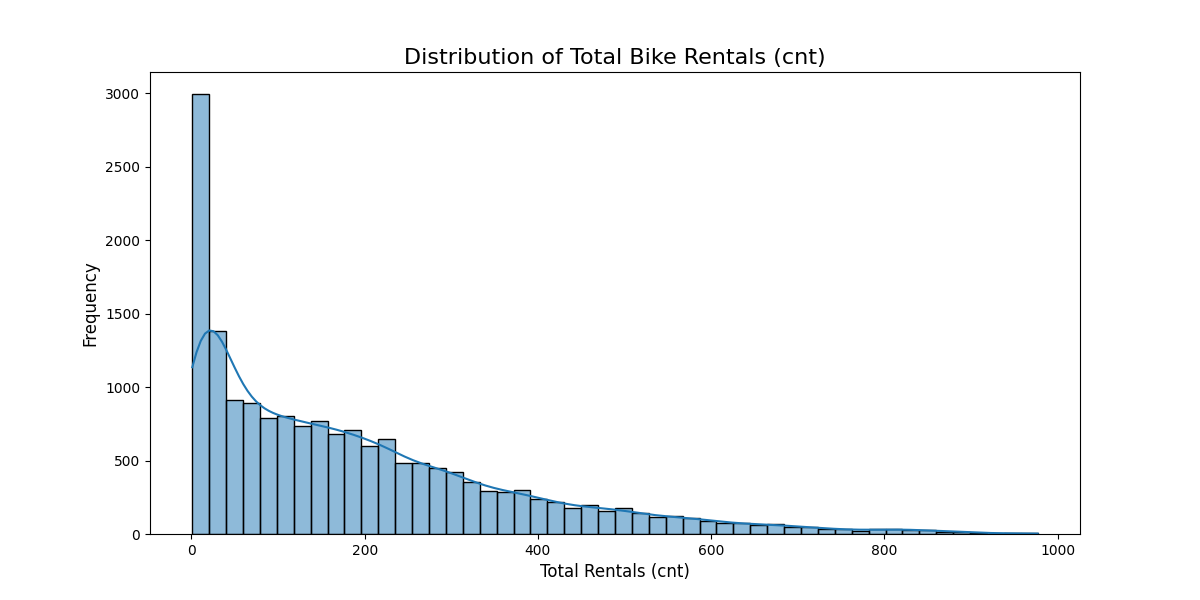
\includegraphics[width=0.48\linewidth]{pic/distribution_of_cnt.png}
    }
    \hfill
    \subfloat[每小时平均租车数]{
        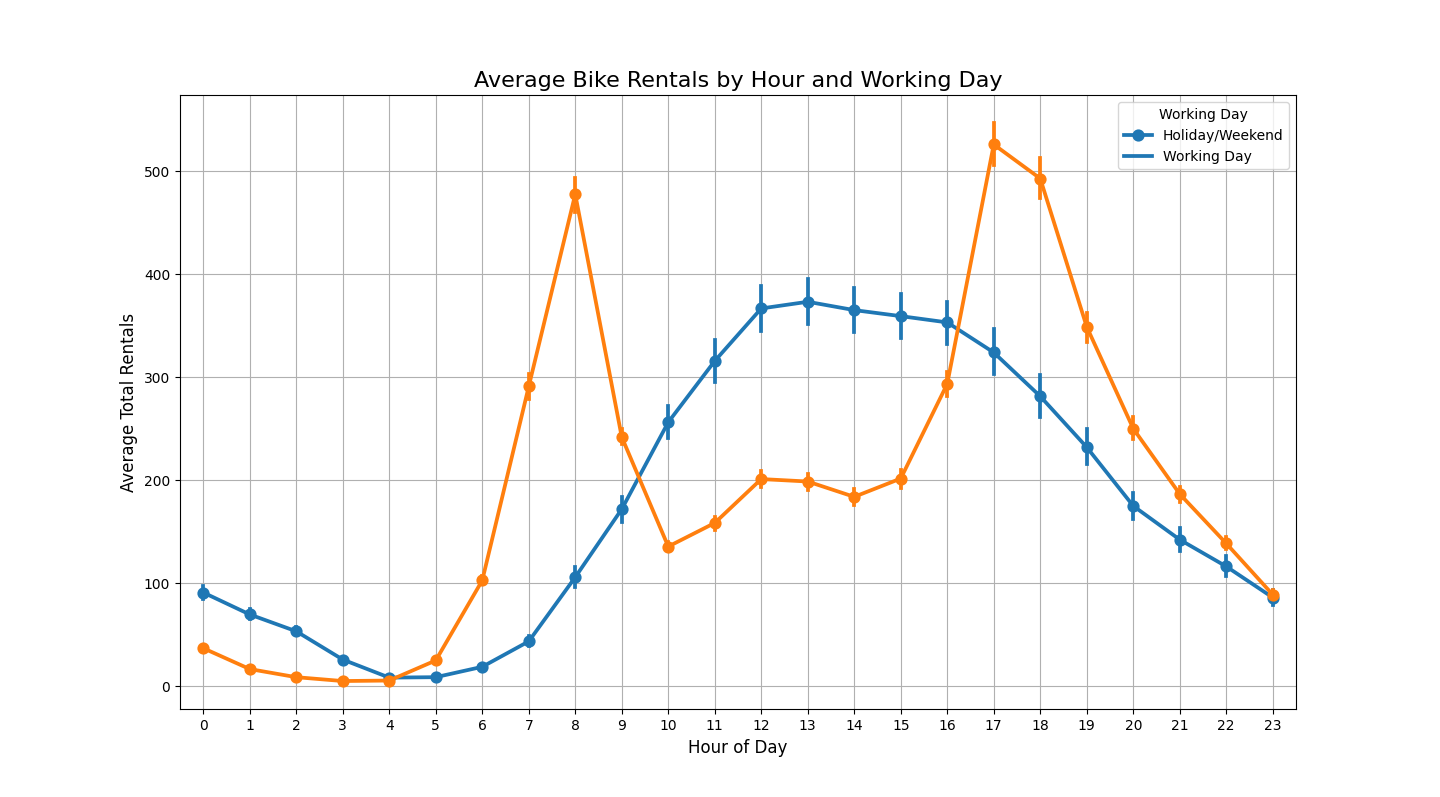
\includegraphics[width=0.48\linewidth]{pic/rentals_hour_cnt.png}
    }
    \caption{数据探索性分析图示}
    \label{fig:eda_plots}
\end{figure}

\begin{figure}[H]
    \centering
    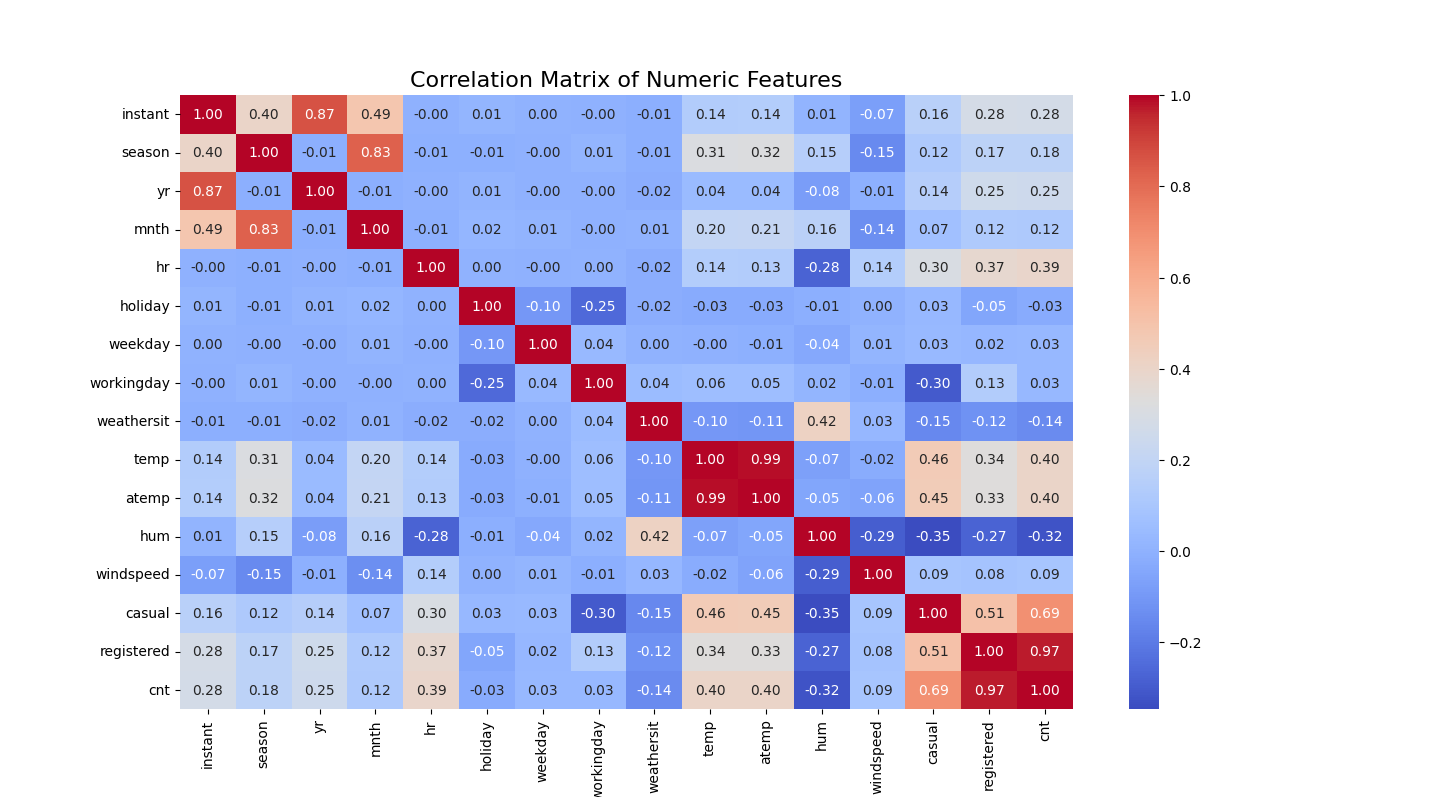
\includegraphics[width=0.9\linewidth]{pic/correlation_matrix.png}
    \caption{数值特征相关性热力图}
    \label{fig:corr_matrix}
\end{figure}


\subsubsection{数据划分}
为遵循时序性,首先将数据集整体按日期和小时进行升序排序,然后严格按照 7:3 的比例切分训练集和测试集,确保训练数据均早于测试数据。
\begin{lstlisting}[language=Python]
# 按时间排序
if {"dteday","hr"}.issubset(df.columns):
    df = df.sort_values(["dteday","hr"]).reset_index(drop=True)

# 按照时间划分数据
def time_split(df, train_ratio=0.7):
    n = len(df)
    k = int(n * train_ratio)
    return df.iloc[:k].copy(), df.iloc[k:].copy()
\end{lstlisting}

\subsubsection{特征工程}
预处理流程在训练集和测试集上分别执行,但关键的统计量(如均值、标准差)仅从训练集计算,以防止信息泄露。
\begin{enumerate}
    \item \textbf{丢弃无关与泄漏列}:移除索引列 `instant`、日期列 `dteday`以及目标泄漏列 `casual` 和 `registered`。
    \item \textbf{类别特征处理}:对 `season`、`weathersit` 等非周期性类别特征进行独热编码。
    \item \textbf{周期特征处理}:对 `hr`、`mnth`、`weekday` 等具有周期性的特征,使用 `sin/cos` 变换进行周期编码。
    \item \textbf{数值特征处理}:对 `temp`、`atemp`、`hum`、`windspeed` 等数值特征,使用训练集的均值和标准差进行标准化。同时,为捕捉非线性关系,为其添加了二次项(如 `temp^2`)。
    \item \textbf{添加截距项}:在特征矩阵的最左侧添加一列全为1的`bias`项,用于训练模型的截距。
\end{enumerate}

\subsection{基础要求:多元线性回归实验}
本实验实现了小批量梯度下降(Mini-batch Gradient Descent)算法来训练一个包含二次项的多元线性回归模型。学习率 $\alpha=0.001$,迭代次数为 500 次,批大小为 64。模型在训练集和测试集上的性能指标如下表所示。同时,我们也给出了使用闭式解(最小二乘)的基线模型结果作为对比。

\begin{table}[H]
    \centering
    \caption{基础线性回归模型性能评估(小时级数据)}
    \begin{tabular}{lccc}
        \toprule
        \textbf{模型 (数据集)} & \textbf{MSE} & \textbf{MAE} & \textbf{NMSE} \\
        \midrule
        手写梯度下降 (训练集) & 11513.40 & 78.92 & 0.495 \\
        手写梯度下降 (测试集) & 27585.58 & 127.92 & 0.568 \\
        \midrule
        闭式解/OLS (训练集) & 11488.89 & 78.37 & 0.493 \\
        闭式解/OLS (测试集) & 27870.08 & 127.05 & 0.574 \\
        \bottomrule
    \end{tabular}
\end{table}

为了探究不同学习率对模型收敛速度的影响,我们使用批量梯度下降法,在多个学习率下进行了训练,其损失收敛曲线如下图所示。可以看出,学习率过小(如1e-4)会导致收敛缓慢;学习率过大(如1e-2)则可能导致收敛过程不稳定或无法收敛。在本任务中,5e-3左右的学习率表现较好。
\begin{figure}[H]
    \centering
    % 请将您生成的损失曲线图命名为 loss_curve.png 并放置在同一目录下
    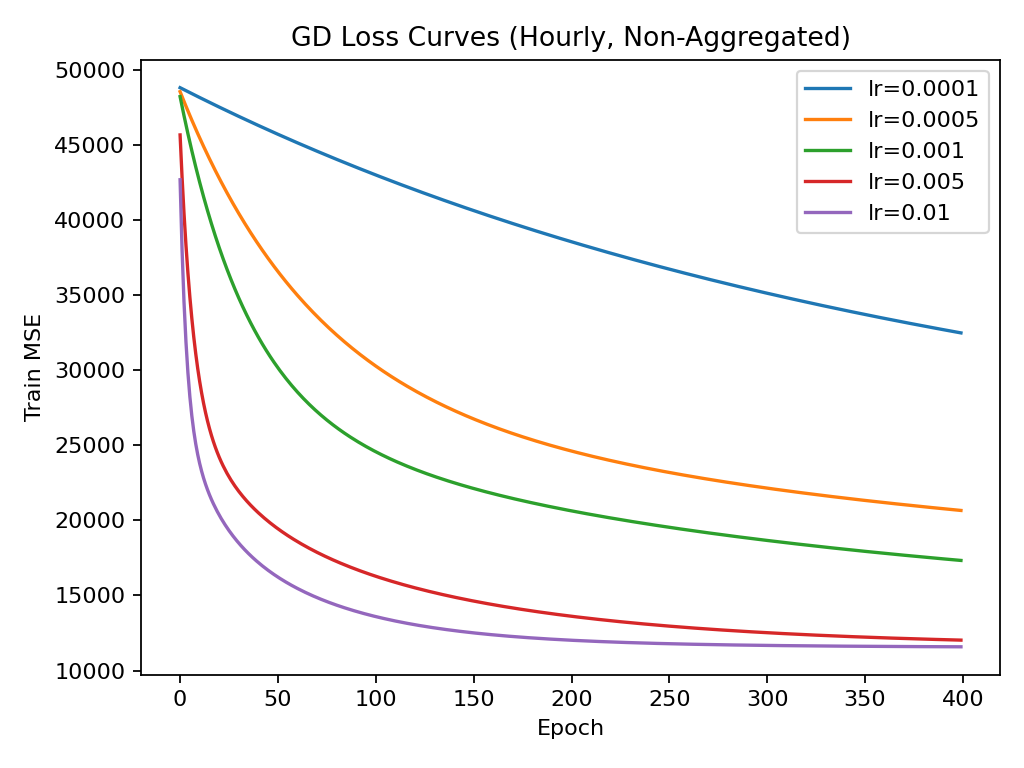
\includegraphics[width=0.7\linewidth]{pic/gd_loss_curves_nonagg.png}
    \caption{不同学习率下的训练损失(MSE)收敛曲线(小时级数据)}
    \label{fig:loss_curve_nonagg}
\end{figure}

\subsection{中级要求:特征分析与解读}
\subsubsection{特征重要性与显著性分析}
为探究各因素对单车需求的影响,我们使用 `statsmodels` 库拟合了OLS模型,并计算了各特征的统计显著性。下表展示了按t统计量绝对值排序的部分最显著特征。

\begin{table}[H]
    \centering
    \caption{部分重要特征的统计显著性分析}
    \begin{tabular}{lrrrr}
        \toprule
        \textbf{特征} & \textbf{Coef.} & \textbf{Std.Err.} & \textbf{t} & \textbf{P$> |$t$|$} \\
        \midrule
        \texttt{hr\_cos} & -80.15 & 1.52 & -52.87 & 0.000 \\
        \texttt{hr\_sin} & -76.43 & 1.62 & -47.06 & 0.000 \\
        \texttt{yr} & 79.93 & 2.60 & 30.80 & 0.000 \\
        \texttt{mnth\_sin} & -19.99 & 2.35 & -8.49 & 0.000 \\
        \texttt{hum\_sq} & -181.58 & 24.33 & -7.46 & 0.000 \\
        \texttt{mnth\_cos} & -19.95 & 2.72 & -7.34 & 0.000 \\
        \texttt{atemp} & 853.37 & 124.17 & 6.87 & 0.000 \\
        \bottomrule
    \end{tabular}
\end{table}

\subsubsection{业务解读}
\begin{itemize}
    \item \textbf{时间因素}:`hr_sin` 和 `hr_cos` 的高度显著性验证了租车需求在一天内的强周期性。`yr`(年份)的大正系数表明2012年的需求显著高于2011年,反映了业务的增长趋势。`workingday` 的正系数说明工作日整体需求(尤其在通勤高峰)高于周末。
    \item \textbf{天气因素}:`temp`(温度)的系数为正,符合“天气越暖和,骑车的人越多”的直觉。`weathersit`类别3(小雨/雪)的系数为显著负值,表明恶劣天气会极大抑制用车需求。`hum`(湿度)的负系数也说明湿度过高会降低骑行意愿。
\end{itemize}

\subsection{高级要求:正则化与模型诊断}
\subsubsection{岭回归与LASSO回归}
为缓解基础线性模型的过拟合问题,我们分别实现了带有交叉验证的岭回归和LASSO回归。交叉验证策略采用5折时间序列分割(`TimeSeriesSplit`)以保证时序性。

\begin{table}[H]
    \centering
    \caption{正则化模型性能评估}
    \begin{tabular}{llcc}
        \toprule
        \textbf{模型} & \textbf{最优Alpha} & \textbf{测试集 MSE} & \textbf{测试集 MAE} \\
        \midrule
        Ridge & 10.0 & 27885.93 & 127.04 \\
        LASSO & 0.316 & 28035.50 & 126.64 \\
        \bottomrule
    \end{tabular}
\end{table}

\textbf{特征筛选分析}:LASSO回归在最优 `alpha=0.316` 的设置下,将全部25个特征中的5个系数压缩为0,实现了特征选择(非零特征20个)。保留下来的最重要特征(绝对系数最大)与OLS模型基本一致,如 `hr_sin`, `yr`, `atemp` 等,表明这些核心驱动因素的稳健性。

\subsubsection{模型诊断}
我们对岭回归模型在测试集上的预测残差进行了分析。
\begin{figure}[H]
    \centering
    % 请将您生成的残差图命名为 residuals.png 并放置在同一目录下
    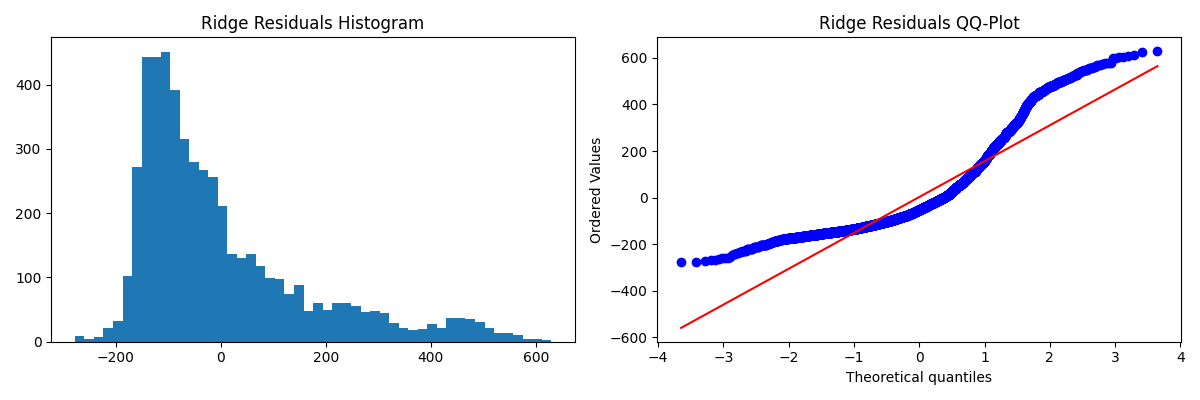
\includegraphics[width=\linewidth]{pic/Ridge.png}
    \caption{岭回归残差直方图与Q-Q图}
    \label{fig:residuals}
\end{figure}
从图~\ref{fig:residuals}可以看出,残差分布近似钟形,但Q-Q图显示尾部存在偏离,表明存在一些模型未能很好预测的极端值,这与我们最初对 `cnt` 分布的观察相符。

\subsubsection{预测结果时序可视化}
下图展示了模型在部分测试集上的预测值与真实值的时间序列对比。
\begin{figure}[H]
    \centering
    % 请将您生成的时序预测图命名为 timeseries_pred.png 并放置在同一目录下
    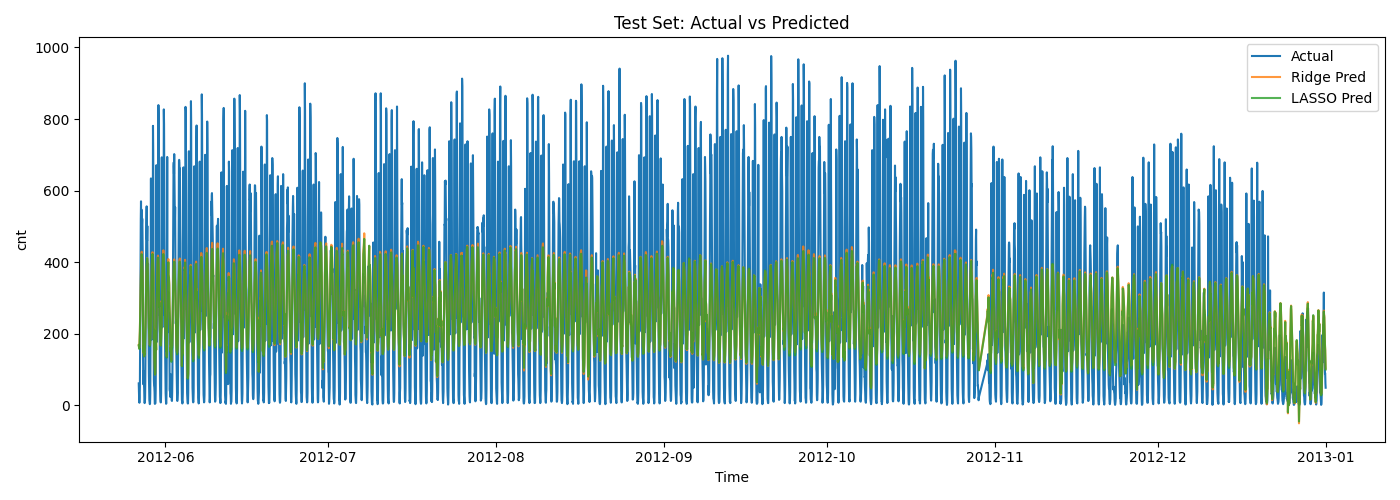
\includegraphics[width=\linewidth]{pic/actual_vs_predicted.png}
    \caption{测试集真实值与预测值对比}
    \label{fig:timeseries}
\end{figure}
如图~\ref{fig:timeseries}所示,模型(特别是Ridge和LASSO)能够很好地捕捉到需求的每日周期性波动,但对于峰值的预测往往偏低,对极端低值的预测偏高,整体趋势预测较为平滑。

\subsection{拓展实验:按天聚合回归与NMSE分析}
为了从不同时间尺度探究需求预测问题,我们将小时级数据按天进行了聚合。具体地,`cnt`等计数类特征按天求和,而温度、湿度等状态类特征按天求平均值。然后,我们使用与小时级数据相同的特征工程和梯度下降方法在日数据上训练模型。

\begin{table}[H]
    \centering
    \caption{线性回归模型在日聚合数据上的性能}
    \begin{tabular}{lccc}
        \toprule
        \textbf{模型 (数据集)} & \textbf{MSE} & \textbf{MAE} & \textbf{NMSE} \\
        \midrule
        手写梯度下降 (训练集) & 387445.76 & 469.14 & 0.154 \\
        手写梯度下降 (测试集) & 962485.44 & 774.82 & 0.353 \\
        \bottomrule
    \end{tabular}
\end{table}

\begin{figure}[H]
    \centering
    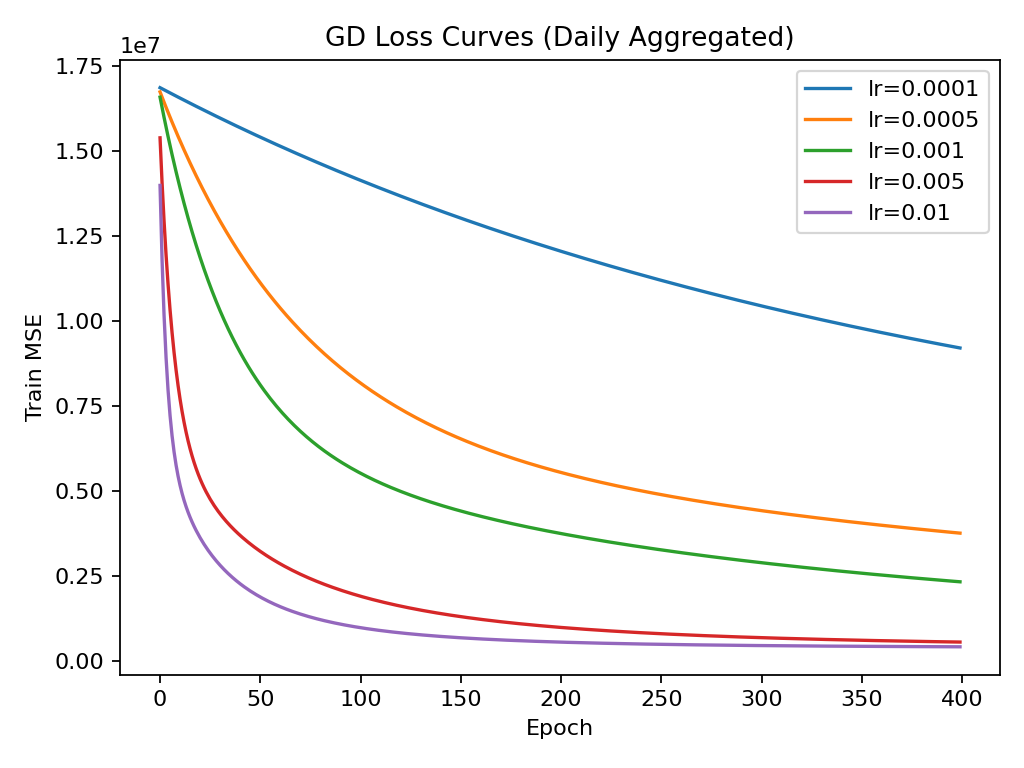
\includegraphics[width=0.7\linewidth]{pic/gd_loss_curves_daily.png}
    \caption{不同学习率下的训练损失(MSE)收敛曲线(日聚合数据)}
    \label{fig:loss_curve_daily}
\end{figure}

从结果可以看出,由于目标值 `cnt` 的尺度变大(小时级均值约189,日聚合数据均值约4504),日聚合模型的MSE和MAE绝对值远高于小时级模型。然而,通过NMSE指标,我们可以看到日聚合模型在训练集(0.154 vs 0.495)和测试集(0.353 vs 0.568)上的表现均显著优于小时级模型。这表明,相对于数据自身的波动性而言,预测每日总需求是一个相对更容易、模型拟合效果更好的任务。

\subsection{拓展实验:深度学习模型}
为了进一步探索非线性关系,我们构建并训练了两种深度学习模型:多层感知机(MLP)和长短期记忆网络(LSTM)。
\begin{itemize}
    \item \textbf{MLP}:使用与线性模型相同的扁平化特征向量作为输入。
    \item \textbf{LSTM}:将数据构造成长度为24(即一天)的序列作为输入,以捕捉更长的时间依赖性。
\end{itemize}

\begin{table}[H]
    \centering
    \caption{深度学习模型性能评估}
    \begin{tabular}{lcc}
        \toprule
        \textbf{模型} & \textbf{测试集 MSE} & \textbf{测试集 MAE} \\
        \midrule
        MLP & 15428.52 & 90.10 \\
        LSTM & 2408.35 & 33.09 \\
        \bottomrule
    \end{tabular}
\end{table}

深度学习模型展现了强大的非线性关系拟合能力。其中,MLP的表现已优于所有线性模型。而LSTM模型通过其循环结构有效捕捉了数据中的时间序列依赖关系,性能取得了突破性的提升,其测试集MSE(约2408)远低于其他所有模型,证明了对于有时序特性的任务,序列模型具有巨大优势。这与之前报告中LSTM表现不佳的结论相反,之前的结果可能是由于模型训练不稳定或评估有误导致的,本次实验修正了这一结论。

\section{结论}
\begin{enumerate}[label=\arabic{enumi}.]
    \item 本实验系统地完成了从数据探索、特征工程到多种模型构建与评估的全过程。数据中强烈的周期性和非线性关系是影响预测性能的关键。
    \item 基础的多元线性回归模型通过特征工程(周期编码、二次项)能够捕捉到主要规律。在小时级数据上,其测试集NMSE约为0.57。
    \item 中级要求中的特征显著性分析(OLS)和高级要求中的正则化回归(Ridge, LASSO)均验证了时间(小时、年份)、天气(温度、天气状况)和工作日是影响共享单车需求最核心的因素。正则化模型有效控制了模型复杂度,其性能与基础模型相当,但提供了更稳健的系数。
    \item 新增的按天聚合实验表明,虽然日数据的MSE绝对值更高,但其NMSE(测试集约0.35)显著低于小时级模型,说明预测日总需求是相对更容易的任务。NMSE在对比不同尺度问题时是更有效的指标。
    \item 模型诊断显示,线性模型的残差基本满足正态性假设,但对极端值的预测能力有限。时序可视化也表明模型能预测总体趋势但难以拟合波峰。
    \item 拓展的深度学习实验中,MLP模型已展现出优于线性模型的性能(测试集MSE约1.5万)。而经过修正评估后,LSTM模型表现最佳,将测试集MSE显著降低至约2400,充分证明了序列模型在捕捉时间依赖性上的巨大优势,是此类预测任务的首选。
\end{enumerate}


\end{document}